\lab{Introduction to Matplotlib}{Matplotlib}
\label{lab:Matplotlib}
\objective{
Matplotlib is the most commonly-used data visualization library in Python. Being able to visualize data helps to determine patterns, to communicate results, and is a key component of applied and computational mathematics.
In this lab we introduce techniques for visualizing data in 1, 2, and 3 dimensions.
The plotting techniques presented here will be used in the remainder of the labs in the manual.
}

\section*{Line Plots} % =======================================================

The quickest way to visualize a simple 1-dimensional array is via a \emph{line plot}.
The following code creates an array of outputs of the function $f(x) = x^2$, then visualizes the array using the \li{matplotlib} module.\footnote{Like NumPy, Matplotlib is \emph{not} part of the Python standard library, but it is included in most Python distributions.}

\begin{lstlisting}
>>> import numpy as np
>>> from matplotlib import pyplot as plt

>>> y = np.arange(-5,6)**2
>>> y
array([25, 16,  9,  4,  1,  0,  1,  4,  9, 16, 25])

# Visualize the plot.
>>> plt.plot(y)                     # Draw the line plot.
<<[<matplotlib.lines.Line2D object at 0x1084762d0>]>>
>>> plt.show()                      # Reveal the resulting plot.
\end{lstlisting}

The result is shown in Figure \ref{fig:basic1}.
Just as \li{np} is a standard alias for NumPy, \li{plt} is a standard alias for \li{matplotlib.pyplot} in the Python community.

The call \li{plt.plot(y)} creates a figure and draws straight lines connecting the entries of \li{y} relative to the $y$-axis.
The $x$-axis is by default the index of the array, namely the integers from $0$ to $10$.
Calling \li{plt.show()} then displays the figure.

\begin{figure}[H] % plt.plot(y) compared to plt.plot(x,y).
\captionsetup[subfigure]{justification=centering}
\centering
\begin{subfigure}{.5\textwidth}
    \centering
    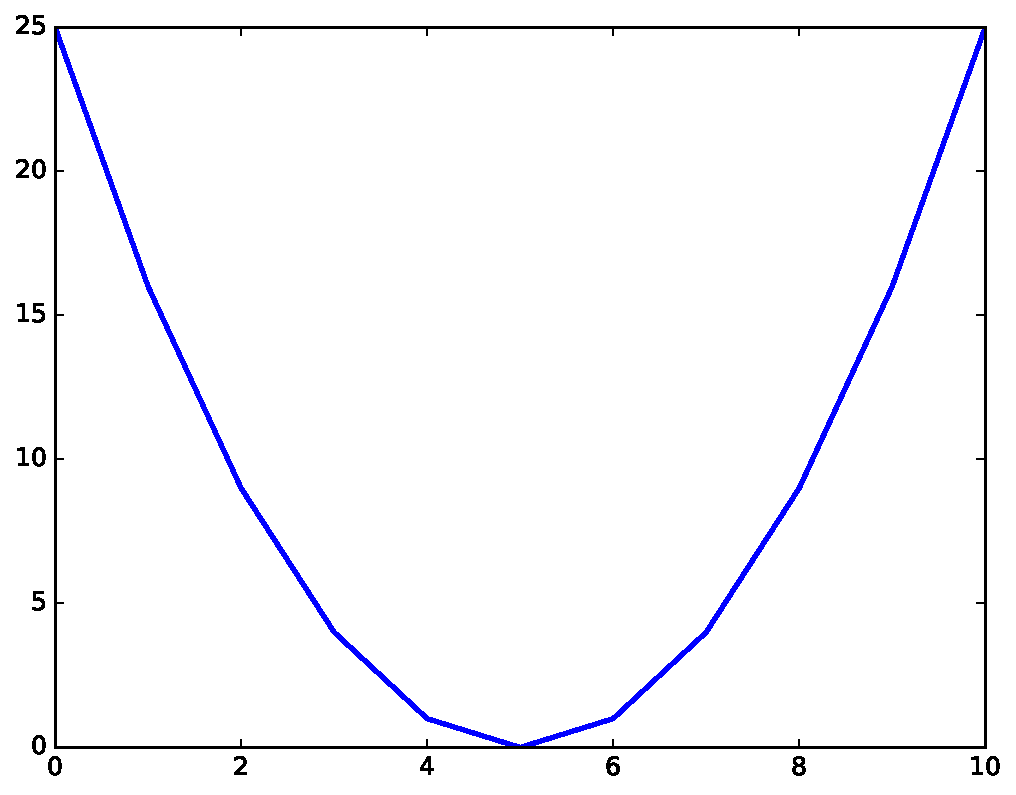
\includegraphics[width=\linewidth]{figures/basic1.pdf}
    \caption{\li{plt.plot(y)} uses the indices of\\the array for the $x$-axis.}
    \label{fig:basic1}
\end{subfigure}%
\begin{subfigure}{.5\textwidth}
    \centering
    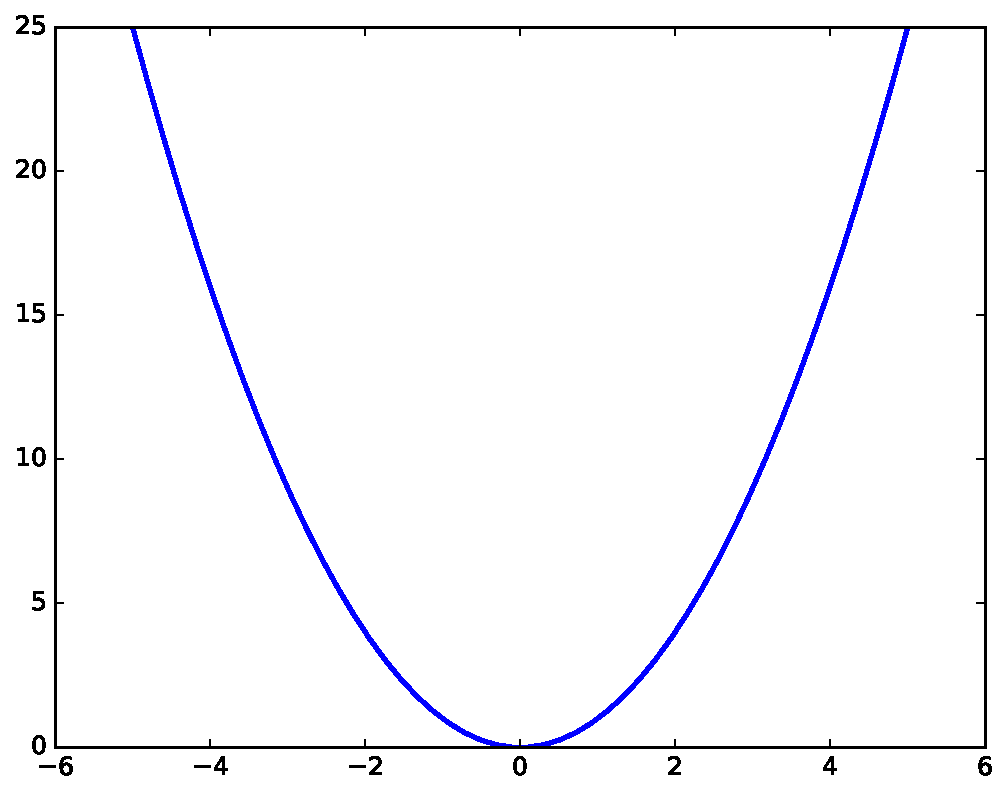
\includegraphics[width=\linewidth]{figures/basic2.pdf}
    \caption{\li{plt.plot(x,y)} specifies both the\\domain and the range.}
    \label{fig:basic2}
\end{subfigure}
\caption{Simple plots of $f(x) = x^2$ over the interval $x\in[-5,5]$.}
\end{figure}

\begin{problem} % Law of Large Numbers / NumPy review.
Write a function that accepts an integer $n$ as input.
\begin{enumerate}
\item Use \li{np.random.randn()} or \li{np.random.normal()} to create an $n\times n$ array of values randomly sampled from the standard normal distribution.
\item Compute the mean of each row of the array.
\\(Hint: use \li{np.mean()} and specify the \li{axis} keyword argument.)
\item Return the variance of these means.
\\(Hint: use \li{np.var()} to calcualte the variance).
\end{enumerate}
Define a new function that creates an array of the results of the first function with inputs $n = 100,\ 200,\ \ldots,\ 1000$.
Plot (and show) the resulting array.

This result illustrates one version of the \emph{Law of Large Numbers}.
\end{problem}

\subsection*{Specifying a Domain} % -----------------------------------------

An obvious problem with Figure \ref{fig:basic1} is that the $x$-axis does not correspond correctly to the $y$-axis for the function $f(x) = x^2$ that is being drawn.
To correct this, we need an array for the domain as well as one for the range.
First define an array \li{x} for the domain, then use that array to calculate the range \li{y} of $f$.
The command \li{plt.plot(x,y)} then plots \li{x} against \li{y}.
That is, each point \li{(x[i], y[i])} is drawn and consecutive points are connected.
% Thus both arrays must have the same number of elements to be compatible.

Another problem with Figure \ref{fig:basic1} is its poor resolution; the curve is visibly bumpy, especially near the bottom of the curve.
NumPy's \li{np.linspace()} function makes it easy to get a higher-resolution domain.
Recall that \li{range()} and \li{np.arange()} return a list or array of evenly-spaced values in a given interval, where the \emph{spacing} between the entries is specified.
In contrast, \li{np.linspace()} creates an array of evenly-spaced values in a given interval where the \emph{number of elements} is specified.

\begin{lstlisting}
# 4 evenly-spaced values between 0 and 32 (including endpoints).
>>> np.linspace(0, 32, 4)
array([  0.        ,  10.66666667,  21.33333333,  32.        ])

# Get 50 evenly-spaced values from -5 to 5 (including endpoints).
>>> x = np.linspace(-5, 5, 50)
>>> y = x**2                        # Calculate the range of f(x) = x**2.
>>> plt.plot(x, y)
>>> plt.show()
\end{lstlisting}

The resulting plot is shown in Figure \ref{fig:basic2}.
Note that this time, the $x$-axis is correctly aligned with the $y$-axis.
The resolution is also much better because \li{x} and \li{y} have $50$ entries each instead of only $10$.

All calls to \li{plt} functions modify the same figure until \li{plt.show()} is executed, which displays the current figure and resets the system.%
\footnote{Use \li{plt.figure()} to manually create several figures at once.}
The next time a \li{plt} function is called a new figure is created.
This makes it possible to plot several lines in a single figure.


\begin{problem} % Plot two lines (sin() and cos()).
Write a function that plots the functions $\sin(x)$, $\cos(x)$, and $\arctan(x)$ on the domain $[-2\pi, 2\pi]$ (use \li{np.pi} for $\pi$).
% Call \li{plt.xlim(-2*np.pi, 2*np.pi)} before \li{plt.show()} to stretch the $x$-axis appropriately.
Make sure the domain is refined enough to produce a figure with good resolution.
\end{problem}

\begin{info} % Interactive Mode.
Plotting can seem a little mystical because the actual plot doesn't appear until \li{plt.show()} is executed.
Matplotlib's \emph{interactive mode} allows the user to see the plot be constructed one piece at a time.
Use \li{plt.ion()} to turn interactive mode on and \li{plt.ioff()} to turn it off.
This is very useful for quick experimentation.

Try executing the following commands in IPython:

\begin{lstlisting}
In [1]: import numpy as np
In [2]: from matplotlib import pyplot as plt

# Turn interactive mode on and make some plots.
In [3]: plt.ion()
In [4]: x = np.linspace(1, 4, 100)
In [5]: plt.plot(x, np.log(x))
In [6]: plt.plot(x, np.exp(x))

# Clear the figure, then turn interactive mode off.
In [7]: plt.clf()
In [8]: plt.ioff()
\end{lstlisting}

Use interactive mode \textbf{only} with IPython.
Using interactive mode in a non-interactive setting may freeze the window or cause other problems.
\end{info}

\section*{Plot Customization} % ===============================================

\li{plt.plot()} receives several keyword arguments for customizing the drawing.
For example, the color and style of the line are specified by the following string arguments.
%
\begin{table}[H] % Color and style.
\begin{tabular}{r|l}
    Key & Color \\
    \hline
    \li{'b'} & blue\\
    \li{'g'} & green\\
    \li{'r'} & red\\
    \li{'c'} & cyan\\
    \li{'m'} & magenta\\
    % \li{'y'} & yellow\\
    \li{'k'} & black\\
    % \li{'w'} & white
\end{tabular}
\qquad
\begin{tabular}{r|l}
    Key & Style \\
    \hline
    \li{'-'} & solid line\\
    \li{'--'} & dashed line\\
    \li{'-.'} & dash-dot line\\
    \li{':'} & dotted line\\
    % \li{'.'} & point marker\\
    \li{'o'} & circle marker\\
    % \li{'*'} & star marker\\
    \li{'+'} & plus marker
\end{tabular}
\end{table}

Specify one or both of these string codes as an argument to \li{plt.plot()} to change from the default color and style.
Other \li{plt} functions further customize a figure.
%
\begin{table}[H]
\centering
\begin{tabular}{r|l}
    Function & \multicolumn{1}{|c}{Description}\\
    \hline
    % \li{grid()} & Add grid lines\\
    \li{legend()} & Place a legend in the plot\\
    % \li{text()} & Add text at a given position on the plot\\
    \li{title()} & Add a title to the plot\\
    \li{xlim()} & Set the limits of the $x$-axis\\
    \li{ylim()} & Set the limits of the $y$-axis\\
    % \li{xticks()} & set the location of the tick marks on the x axis, returns current locations if no arguments are given\\
    % \li{yticks()} & set the location of the tick marks on the y axis, returns current locations if no arguments are given\\
    \li{xlabel()} & Add a label to the $x$-axis\\
    \li{ylabel()} & Add a label to the $y$-axis
\end{tabular}
\end{table}

\begin{lstlisting}
>>> x1 = np.linspace(-2, 4, 100)
>>> plt.plot(x1, np.exp(x1), 'g:', linewidth=6, label="Exponential")
>>> plt.title("This is the title.", fontsize=18)
>>> plt.legend(loc="upper left")    # plt.legend() uses the 'label' argument of
>>> plt.show()                      # plt.plot() to create a legend.

>>> x2 = np.linspace(1, 4, 100)
>>> plt.plot(x2, np.log(x2), 'r+', markersize=4)
>>> plt.xlim(0, 5)                  # Set the visible limits of the x axis.
>>> plt.xlabel("The x axis")        # Give the x axis a label.
>>> plt.show()
\end{lstlisting}

\begin{figure}[H] % Figure customizations.
\captionsetup[subfigure]{justification=centering}
\centering
\begin{subfigure}{.49\textwidth}
    \centering
    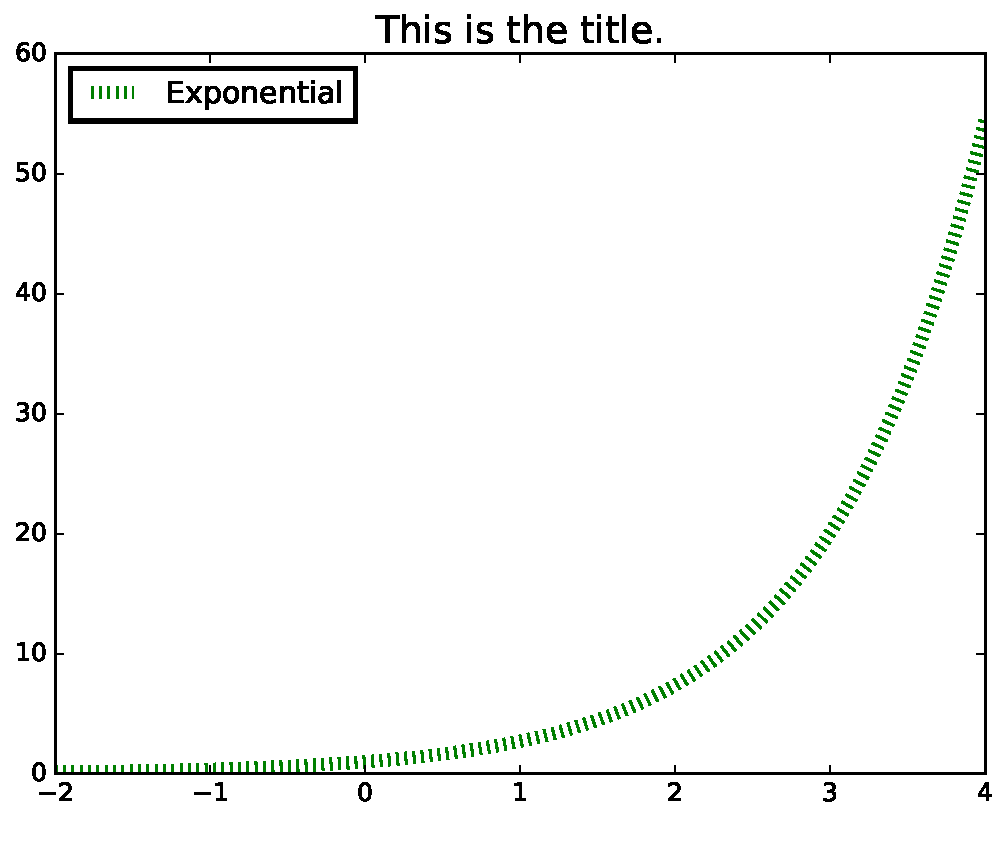
\includegraphics[width=\linewidth]{figures/custom1.pdf}
    \label{fig:custom1}
\end{subfigure}
%
\begin{subfigure}{.49\textwidth}
    \centering
    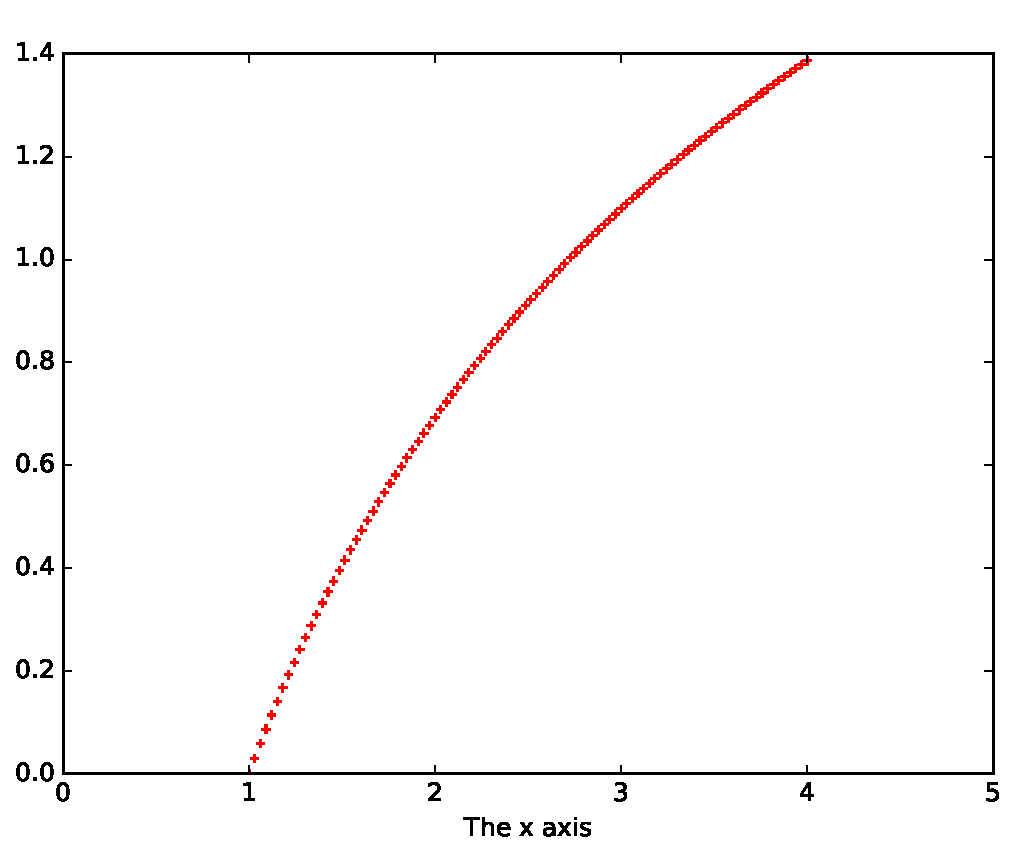
\includegraphics[width=\linewidth]{figures/custom2.pdf}
    \label{fig:custom2}
\end{subfigure}
\label{fig:custom}
\end{figure}

See Appendix \ref{mpltables} for more comprehensive lists of colors, line styles, and figure customization routines.

\begin{problem} % Line plots with different domains but uniform style.
Write a function to plot the curve $f(x) = \frac{1}{x-1}$ on the domain $[-2,6]$.
Although $f(x)$ has a discontinuity at $x=1$, a single call to \li{plt.plot()} will attempt to make the curve look continuous.
\begin{enumerate}
\item Split up the domain and plot the two sides of the curve separately so that the graph looks discontinuous at $x=1$.
\item Plot both curves with a thick, dashed magenta line.\\
The keyword arguments \li{linewidth} or \li{lw} specify the line thickness.
\item Change the range of the $y$-axis to be $[-6, 6]$.
\end{enumerate}
The plot should resemble the figure below.

\begin{figure}[H] % Solution.
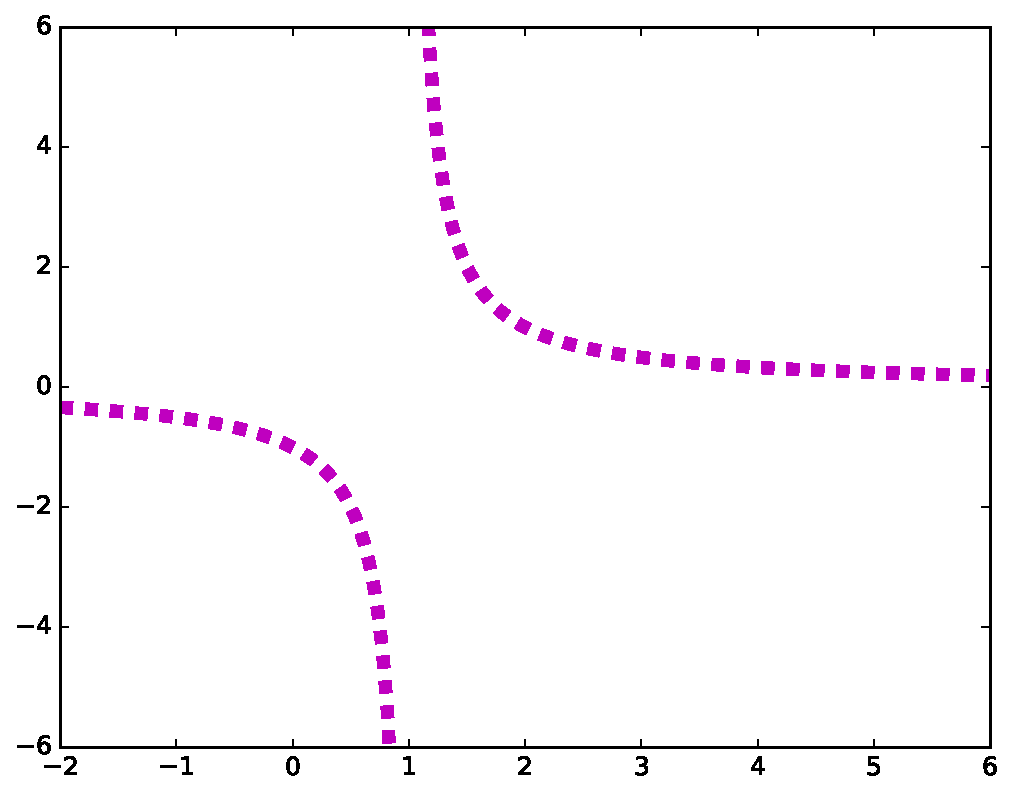
\includegraphics[width=.5\textwidth]{figures/discontinuousProblem.pdf}
\end{figure}
\end{problem}

\subsection*{Subplots} % ------------------------------------------------------

\emph{Subplots} are non-overlapping plots arranged in a grid within a single figure.
To create a figure with a grid of subplots, use \li{plt.subplot(numrows, numcols, fignum)}.
Here, \li{numrows} is the number of rows of subplots in the figure, \li{numcols} is the number of columns, and \li{fignum} specifies which subplot to modify.
% This index starts at 1 and increments across rows first.
See Figure \ref{fig:subplots-layout}.

\begin{figure}[H] % The layout created by subplots(23i).
\captionsetup[subfigure]{justification=centering}
\centering
\begin{subfigure}{.15\textwidth}
    \centering
    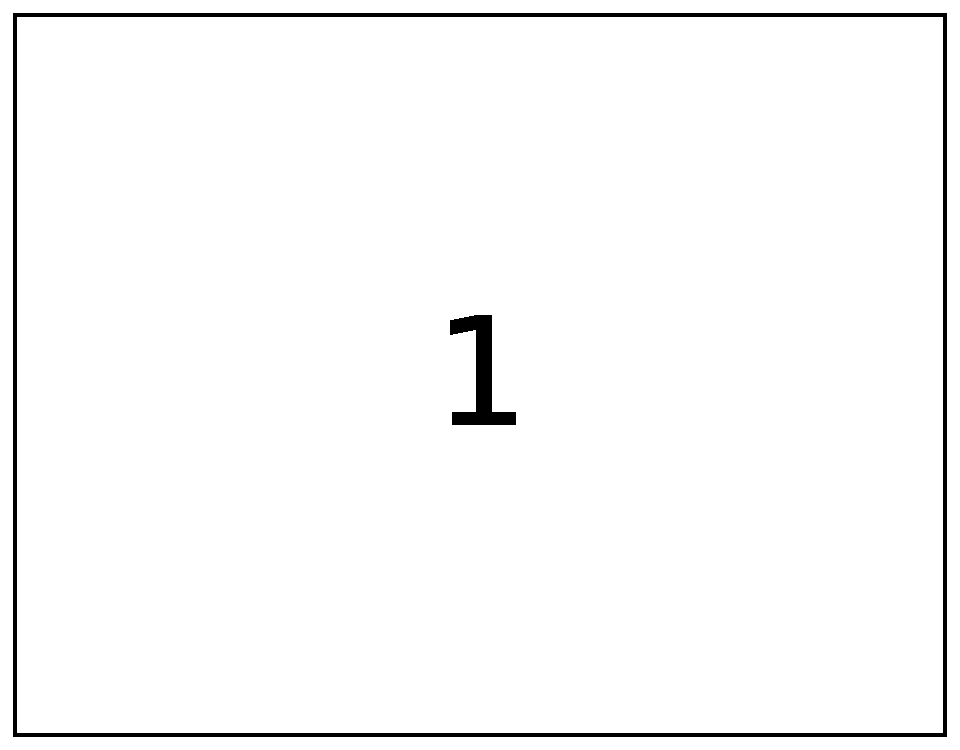
\includegraphics[width=\linewidth]{figures/layout_1.pdf}
\end{subfigure}
%
\begin{subfigure}{.15\textwidth}
    \centering
    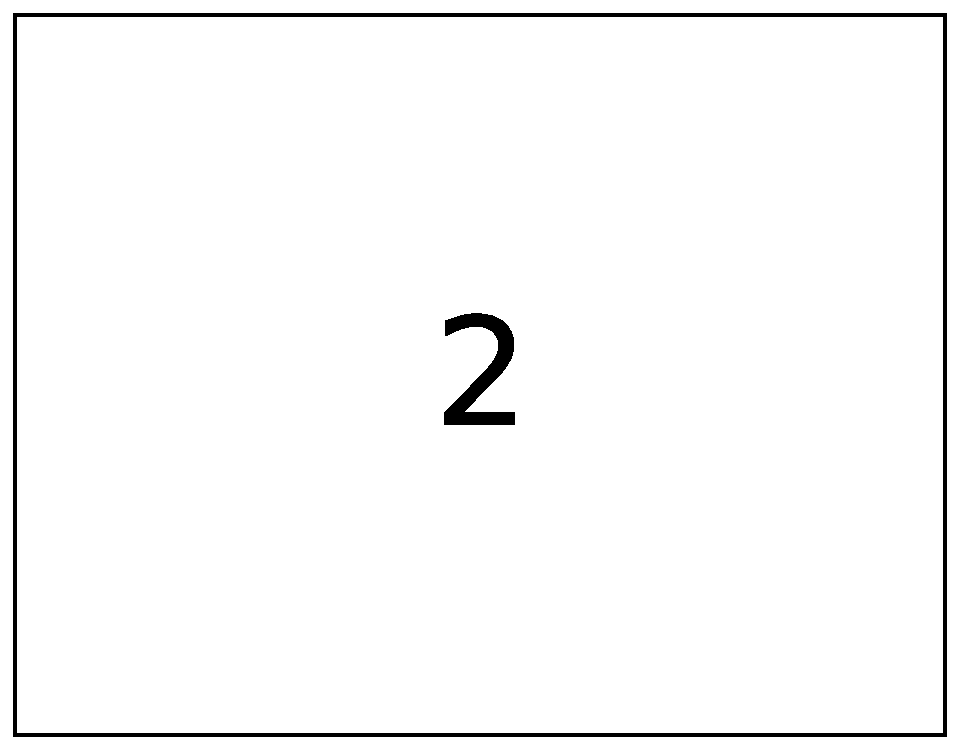
\includegraphics[width=\linewidth]{figures/layout_2.pdf}
\end{subfigure}
%
\begin{subfigure}{.15\textwidth}
    \centering
    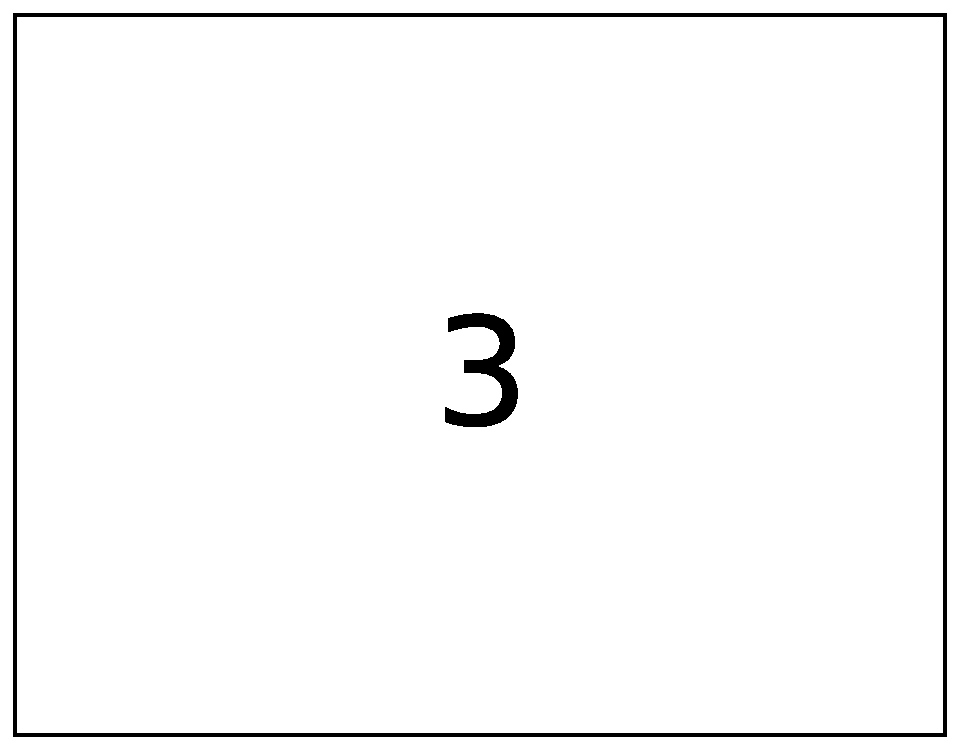
\includegraphics[width=\linewidth]{figures/layout_3.pdf}
\end{subfigure}
\\
\begin{subfigure}{.15\textwidth}
    \centering
    
\includegraphics[width=\linewidth]{figures/layout_4.pdf}
\end{subfigure}
%
\begin{subfigure}{.15\textwidth}
    \centering
    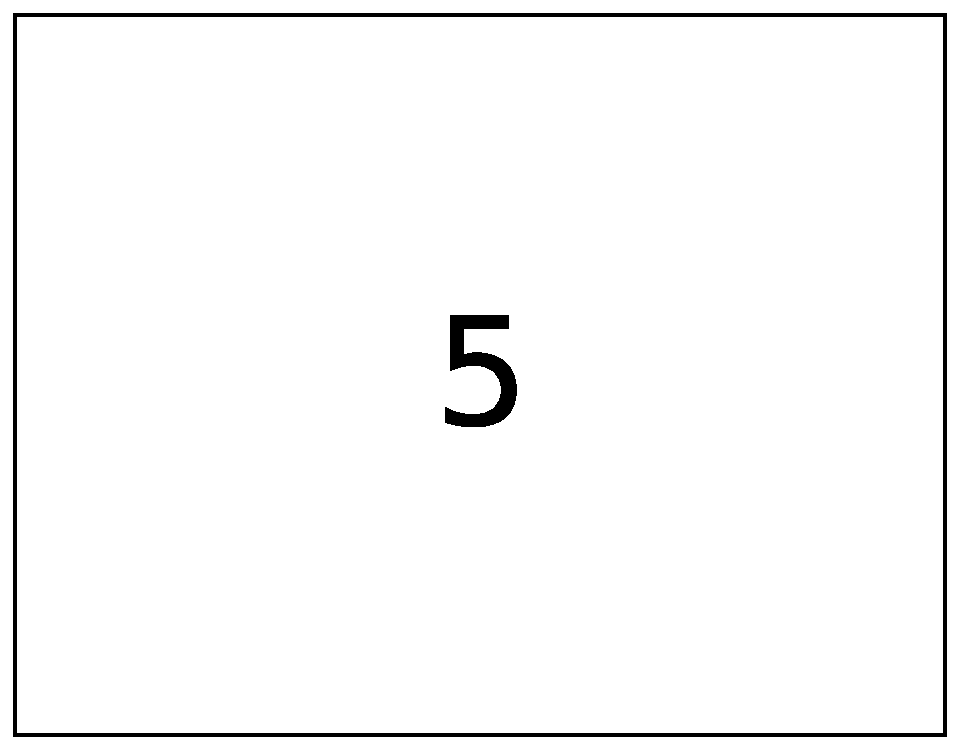
\includegraphics[width=\linewidth]{figures/layout_5.pdf}
\end{subfigure}
%
\begin{subfigure}{.15\textwidth}
    \centering
    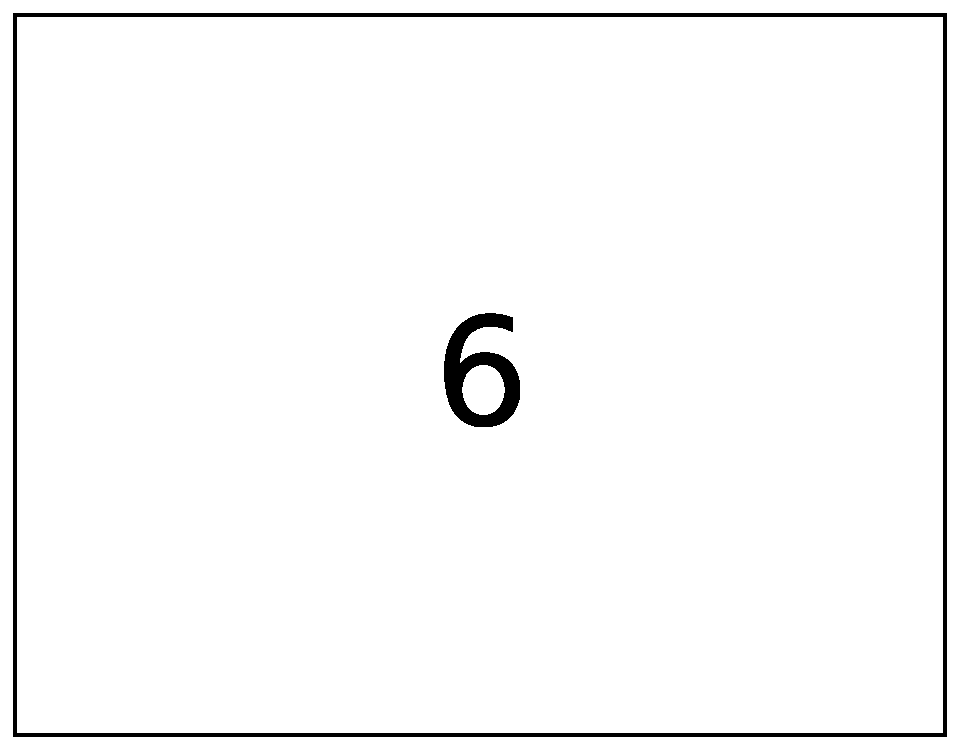
\includegraphics[width=\linewidth]{figures/layout_6.pdf}
\end{subfigure}
\caption{The layout of subplots with \li{plt.subplot(2,3,i)} (2 rows, 3 columns), where \li{i} is the index pictured above.}
\label{fig:subplots-layout}
\end{figure}

If the inputs for \li{plt.subplot()} are all integers, the commas between the entries can be omitted.
For example, \li{plt.subplot(3,2,2)} and \li{plt.subplot(322)} are equivalent.

\begin{lstlisting}
>>> x = np.linspace(.1, 2, 200)

>>> plt.subplot(121)                # Start drawing the first subplot.
>>> plt.plot(x, np.exp(x), 'k', lw=2)
>>> plt.plot(x, np.exp(2*x), 'b', lw=2)
>>> plt.title("Exponential", fontsize=18)

>>> plt.subplot(122)                # Start drawing the second subplot.
>>> plt.plot(x, np.log(x), 'k', lw=2)
>>> plt.plot(x, np.log(2*x), 'b', lw=2)
>>> plt.title("Logarithmic", fontsize=18)

>>> plt.show()
\end{lstlisting}

\begin{figure}[H] % The layout created by plt.subplot(23i).
\captionsetup[subfigure]{justification=centering}
\centering
\begin{subfigure}{.49\textwidth}
    \centering
    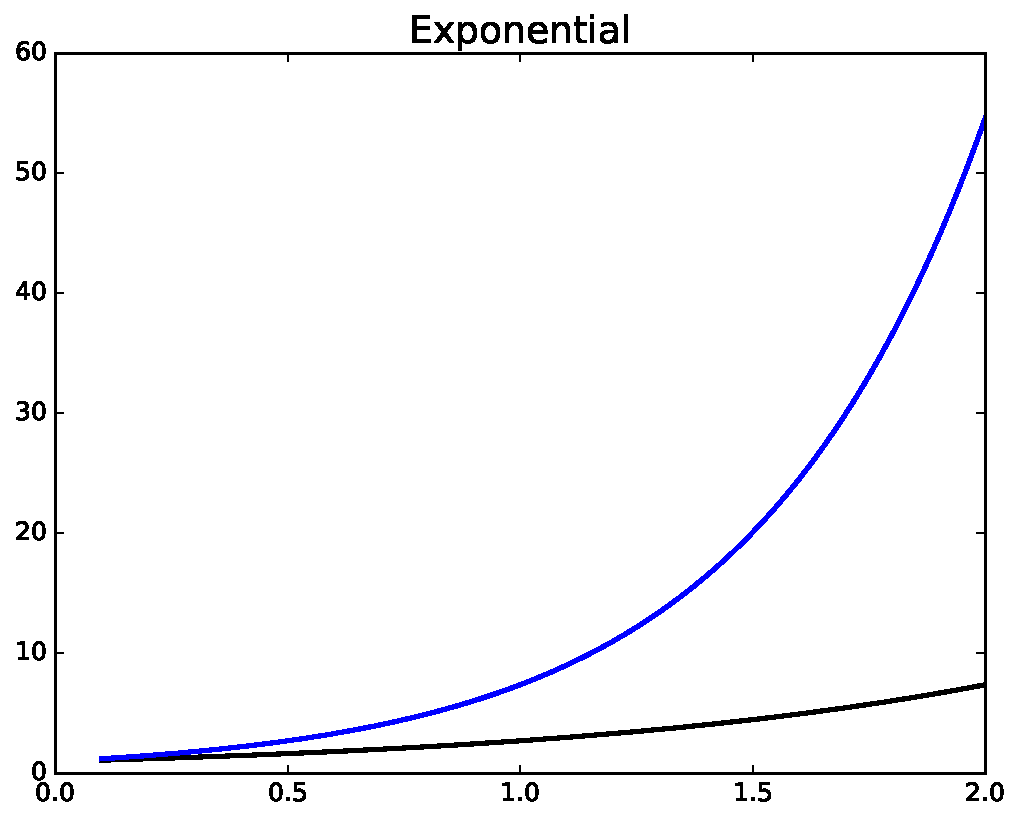
\includegraphics[width=\linewidth]{figures/subplots_1.pdf}
\end{subfigure}
%
\begin{subfigure}{.49\textwidth}
    \centering
    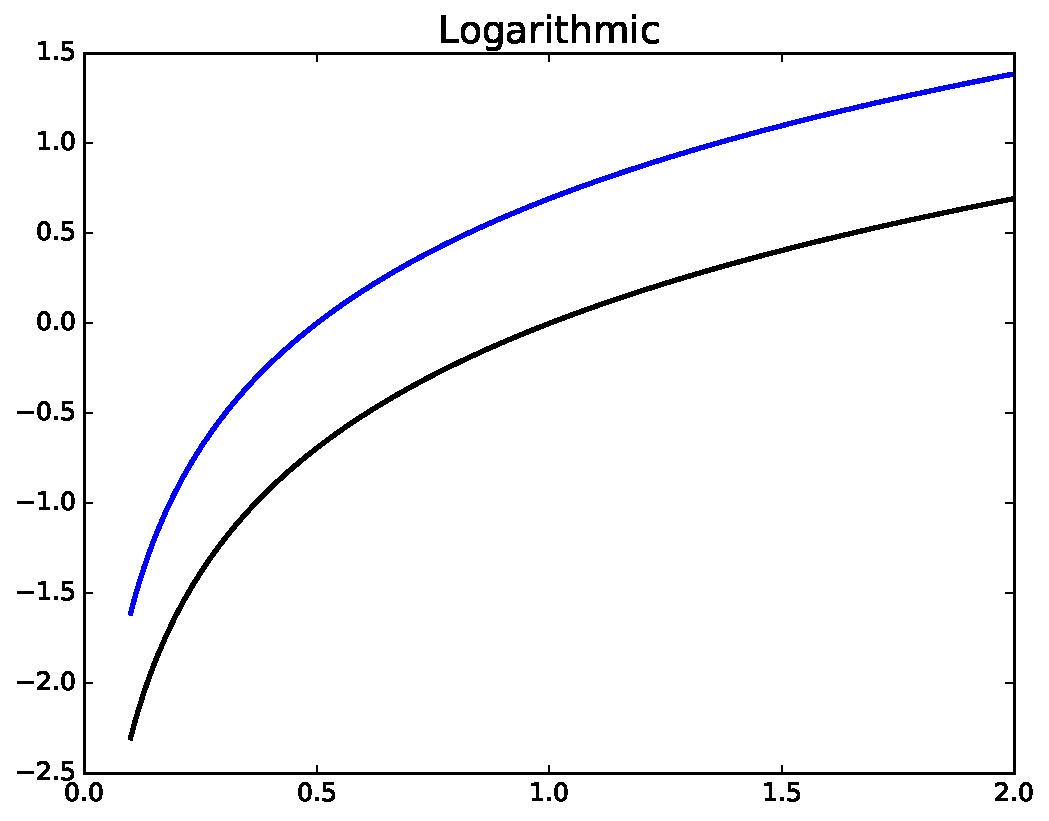
\includegraphics[width=\linewidth]{figures/subplots_2.pdf}
\end{subfigure}
\end{figure}

\begin{problem} % Subplots of sine functions.
Write a function that plots the functions $\sin(x)$, $\sin(2x)$, $2\sin(x)$, and $2\sin(2x)$ on the domain $[0, 2\pi]$, each in a separate subplot.
\begin{enumerate}
    \item Arrange the plots in a square grid of 4 subplots.
    \item Set the limits of each subplot to $[0, 2\pi]\times[-2,2]$.
    \\(Hint: \li{plt.axis()} can do this in one line, instead of using both
    \\\li{plt.xlim()} and \li{plt.ylim()}.)
    \item Use \li{plt.title()} to give each subplot an appropriate title.
    \item Use \li{plt.suptitle()} to give the overall figure a title.
    \item Use the following colors and line styles.
    \begin{align*}\begin{array}{rcl}
    \sin(x)\text{: green solid line.} && \sin(2x)\text{: red dashed line.}\\ \\
    2\sin(x)\text{: blue dashed line.} && 2\sin(2x)\text{: magenta dotted line.}
    \end{array}\end{align*}
\end{enumerate}
\end{problem}

\section*{Other Kinds of Plots} % =============================================

Line plots are not always the most illuminating choice graph to describe a set of data.
Matplotlib provides several other easy ways to visualize data.

\begin{itemize}
\item A \emph{scatter plot} plots two 1-dimensional arrays against each other without drawing lines between the points.
Scatter plots are particularly useful for data that is not inherently correlated or ordered.

To create a scatter plot, use \li{plt.plot()} and specify a point marker (such as \li{'o'} or \li{'+'}) for the line style.%
\footnote{\li{plt.scatter()} can also be used to create scatter plots, but it accepts slightly different arguments than \li{plt.plot()}. We will explore the appropriate usage of this function in a later lab.}

\item A \emph{histogram} groups entries of a 1-dimensional data set into a given number of intervals, called \emph{bins}.
Each bin has a bar whose height indicates the number of values that fall in the range of the bin.
% The more bins, the greater the detail, but having too many bins can also destroy the picture by creating interval gaps between values.
Histograms are best for displaying distributions, relating data values to frequency.

To create a histogram, use \li{plt.hist()} instead of \li{plt.plot()}.
Use the argument \li{bins} to specify the edges of the bins, or to choose a number of bins.
The \li{<<range>>} argument specifies the outer limits of the first and last bins.
\end{itemize}

\begin{lstlisting}
# Get 500 random samples from two normal distributions.
>>> x = np.random.normal(scale=1.5, size=500)
>>> y = np.random.normal(scale=0.5, size=500)

# Draw a scatter plot of x against y, using a circle marker.
>>> plt.subplot(121)
>>> plt.plot(x, y, 'o', markersize=10)

# Draw a histogram to display the distribution of the data in x.
>>> plt.subplot(122)
>>> plt.hist(x, bins=np.arange(-4.5, 5.5))      # Or, equivalently,
#   plt.hist(x, bins=9, range=[-4.5, 4.5])

>>> plt.show()
\end{lstlisting}

\begin{figure}[H]
\captionsetup[subfigure]{justification=centering}
\centering
\begin{subfigure}{.49\textwidth}
    \centering
    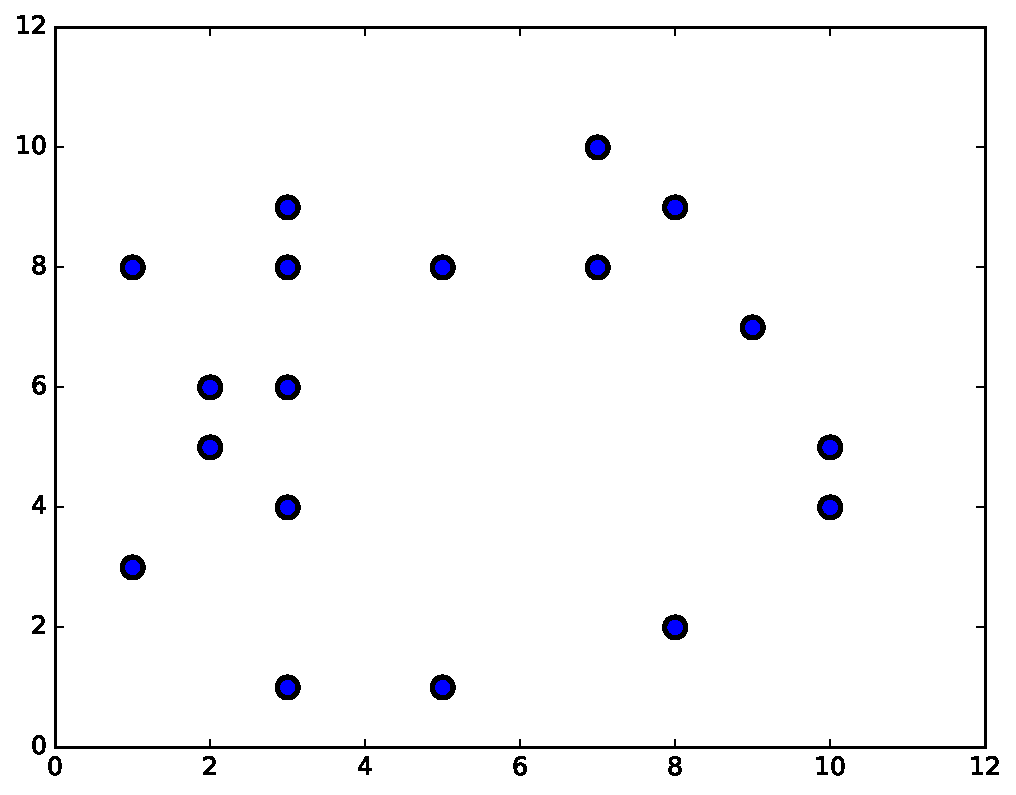
\includegraphics[width=\linewidth]{figures/scatterplot.pdf}
\end{subfigure}
%
\begin{subfigure}{.49\textwidth}
    \centering
    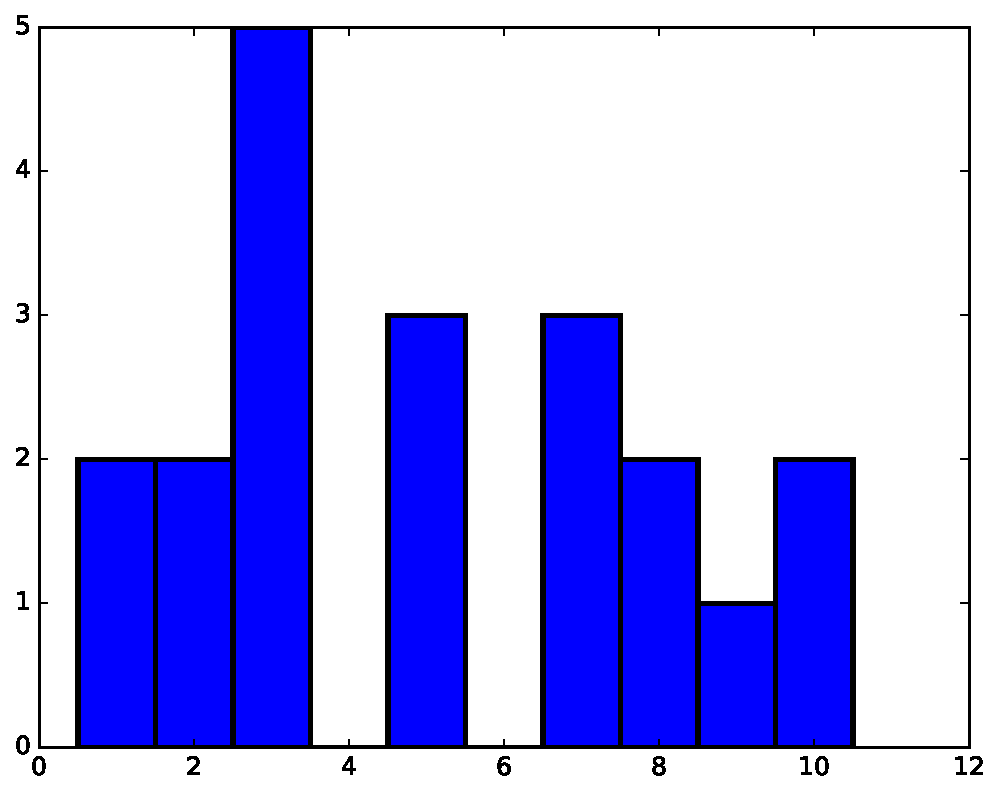
\includegraphics[width=\linewidth]{figures/histogram.pdf}
\end{subfigure}
\end{figure}

% On the histogram, specifying 9 bins in the range $[-4.5, 4.5]$ creates a bin centered over each integer from $-4$ to $4$.

\begin{problem} % FARS data visualization.
The Fatality Analysis Reporting System (FARS) is a nationwide census providing yearly data regarding fatal injuries suffered in motor vehicle traffic crashes.%
\footnote{See \url{http://www.nhtsa.gov/FARS}.}
The array contained in \texttt{FARS.npy} is a small subset of the FARS database from 2010--2014.
Each of the 148,206 rows in the array represents a different car crash; the columns represent the hour (in military time, as an integer), the longitude, and the latitude, in that order.

Write a function to visualize the data in \texttt{FARS.npy}.
Use \li{np.load()} to load the data, then create a single figure with two subplots:
%
\begin{enumerate}
\item A scatter plot of longitudes against latitudes.
Because of the large number of data points, use black pixel markers (use \li{"k,"} as the third argument to \li{plt.plot()}).
Label both axes.
\\
(Hint: Use \li{plt.gca().set_aspect("equal")} to equalize the axes on the scatter plot).

\item A histogram of the hours of the day, with one bin per hour.
Set the limits of the $x$-axis appropriately.
Label the $x$-axis.
\end{enumerate}
\end{problem}

% Other kinds of plots for 1-dimensional data includes bar plots, box plots, and others.
% See Appendix \ref{mpltables} for examples and syntax.

\subsection*{Visualizing 3-D Surfaces} % --------------------------------------

To plot a function $f: \mathbb{R}^2 \rightarrow \mathbb{R}$, we must choose and construct a 2-dimensional domain, then calculate the function at each point of that domain.
The standard tool for creating a 2-dimensional domain in the Cartesian plane is \li{np.meshgrid()}.
Given two 1-dimensional coordinate arrays, \li{np.meshgrid()} creates two corresponding coordinate matrices.
%
\begin{figure}[H] % np.meshgrid() visual demonstration.
\begin{tikzpicture}[>=stealth', shorten <= .1cm,shorten >=.1cm, dot/.style=
    {circle,fill=black,minimum size=3pt,inner sep=0pt, outer sep=-1pt} ]

\foreach \x/\y in {0/0, 0/2, 0/4, 2/0, 2/2, 2/4, 4/0, 4/2, 4/4}
    \node[draw, dot]at(\x,\y){};
\foreach \x/\y in {0/0, 0/1, 0/2, 1/0, 1/1, 1/2, 2/0, 2/1, 2/2}
    \node[draw=none]at(\x*2-.5, \y*2+.3){(\x,\y)};

\foreach \x/\y in {0/0, 0/1, 0/2, 1/0, 1/1, 1/2, 2/0, 2/1, 2/2}
    \node[draw=none]at(\x*.75+7, \y*.75+.1){\y};
\foreach \x/\y in {0/0, 0/1, 0/2, 1/0, 1/1, 1/2, 2/0, 2/1, 2/2}
    \node[draw=none]at(\x*.75+7, \y*-.75+3.9){\x};

\draw[-, thick](6.7,-.25)--(6.7,1.95);
\draw[-, thick](8.8,-.25)--(8.8,1.95);
\draw[-, thick](6.7,2.05)--(6.7,4.25);
\draw[-, thick](8.8,2.05)--(8.8,4.25);
\draw[-, thick](8.8,4.14)--(8.7,4.14);
\draw[-, thick](8.8,2.16)--(8.7,2.16);
\draw[-, thick](6.7,4.14)--(6.8,4.14);
\draw[-, thick](6.7,2.16)--(6.8,2.16);
\draw[-, thick](8.8,1.84)--(8.7,1.84);
\draw[-, thick](8.8,-.135)--(8.7,-.135);
\draw[-, thick](6.8,1.84)--(6.7,1.84);
\draw[-, thick](6.8,-.135)--(6.7,-.135);

\node[draw=none](X)at(6.3,.9){\texttt{Y}=};
\node[draw=none](y)at(6.3,3.15){\texttt{X}=};

\node[draw=none](point1)at(-.3, -.6){\texttt{x}=\big[0,};
\node[draw=none, node distance=2.35cm](point2)
    [right of=point1]{1,};
\node[draw=none, node distance=2cm](point3)
    [right of=point2]{2\big]};
\node[draw=none, rotate=270](point4)at(4.6,4.25)
    {\texttt{y}=\big[2,};
\node[draw=none, rotate=270, node distance=2.35cm](point5)
    [right of=point4]{1,};
\node[draw=none, rotate=270, node distance=2cm](point6)
    [right of=point5]{0\big]};
\end{tikzpicture}
\caption{\li{np.meshgrid(x, y)}, returns the arrays \li{X} and \li{Y}.
The returned arrays give the $x$- and $y$-coordinates of the points in the grid formed by \li{x} and \li{y}.
Specifically, the arrays \li{X} and \li{Y} satisfy \li{(X[i,j], Y[i,j]) = (x[i],y[j])}.}
\label{fig:meshgrid}
\end{figure}

With a 2-dimensional domain, we usually visualize $f$ with two kinds of plots.

\begin{itemize}
\item A \emph{heat map} assigns a color to each entry in the matrix, producing a 2-dimensional picture describing a 3-dimensional shape.
Darker colors typically correspond to lower values while lighter colors typically correspond to higher values.

Use \li{plt.pcolormesh()} to create a heat map.

\item A \emph{contour map} draws several \emph{level curves} of $f$.
A level curve corresponding to the constant $c$ is the collection of points $\left\{(x,y)\mid c = f(x,y)\right\}$.
Coloring the space between the level curves produces a discretized version of a heat map.
Including more and more level curves makes a filled contour plot look more and more like the complete, blended heat map.

Use \li{plt.contour()} to create a contour plot and \li{plt.contourf()} to create a filled contour plot.
Specify either the number of level curves to draw, or a list of constants corresponding to specific level curves.
\end{itemize}

These three functions all receive the keyword argument \li{cmap} to specify a color scheme (some of the better schemes are \li{"viridis"}, \li{"magma"}, and \li{"Spectral"}).
See \url{http://matplotlib.org/examples/color/colormaps_reference.html} for the list of all Matplotlib color schemes.

Finally, to see how the colors in these plots relate to the values of the function, use \li{plt.colorbar()} to draw the color scale beside the plot.

\begin{lstlisting}
# Create a 2-D domain with np.meshgrid().
>>> x = np.linspace(-np.pi, np.pi, 100)
>>> y = x.copy()
>>> X, Y = np.meshgrid(x, y)

# Calculate z = f(x,y) = sin(x)sin(y) using the meshgrid coordinates.
>>> Z = np.sin(X) * np.sin(Y)

# Plot the heat map of f over the 2-D domain.
>>> plt.subplot(131)
>>> plt.pcolormesh(X, Y, Z, cmap="viridis")
>>> plt.colorbar()
>>> plt.xlim(-np.pi, np.pi)
>>> plt.ylim(-np.pi, np.pi)

# Plot a contour map of f with 10 level curves.
>>> plt.subplot(132)
>>> plt.contour(X, Y, Z, 10, cmap="Spectral")
>>> plt.colorbar()

# Plot a filled contour map, specifying the level curves.
>>> plt.subplot(133)
>>> plt.contourf(X, Y, Z, [-1, -.8, -.5, 0, .5, .8, 1], cmap="magma")
>>> plt.colorbar()

>>> plt.show()
\end{lstlisting}

\begin{figure}[H] % heat map and contour plots.
\captionsetup[subfigure]{justification=centering}
\centering
\begin{subfigure}{.33\textwidth}
    \centering
    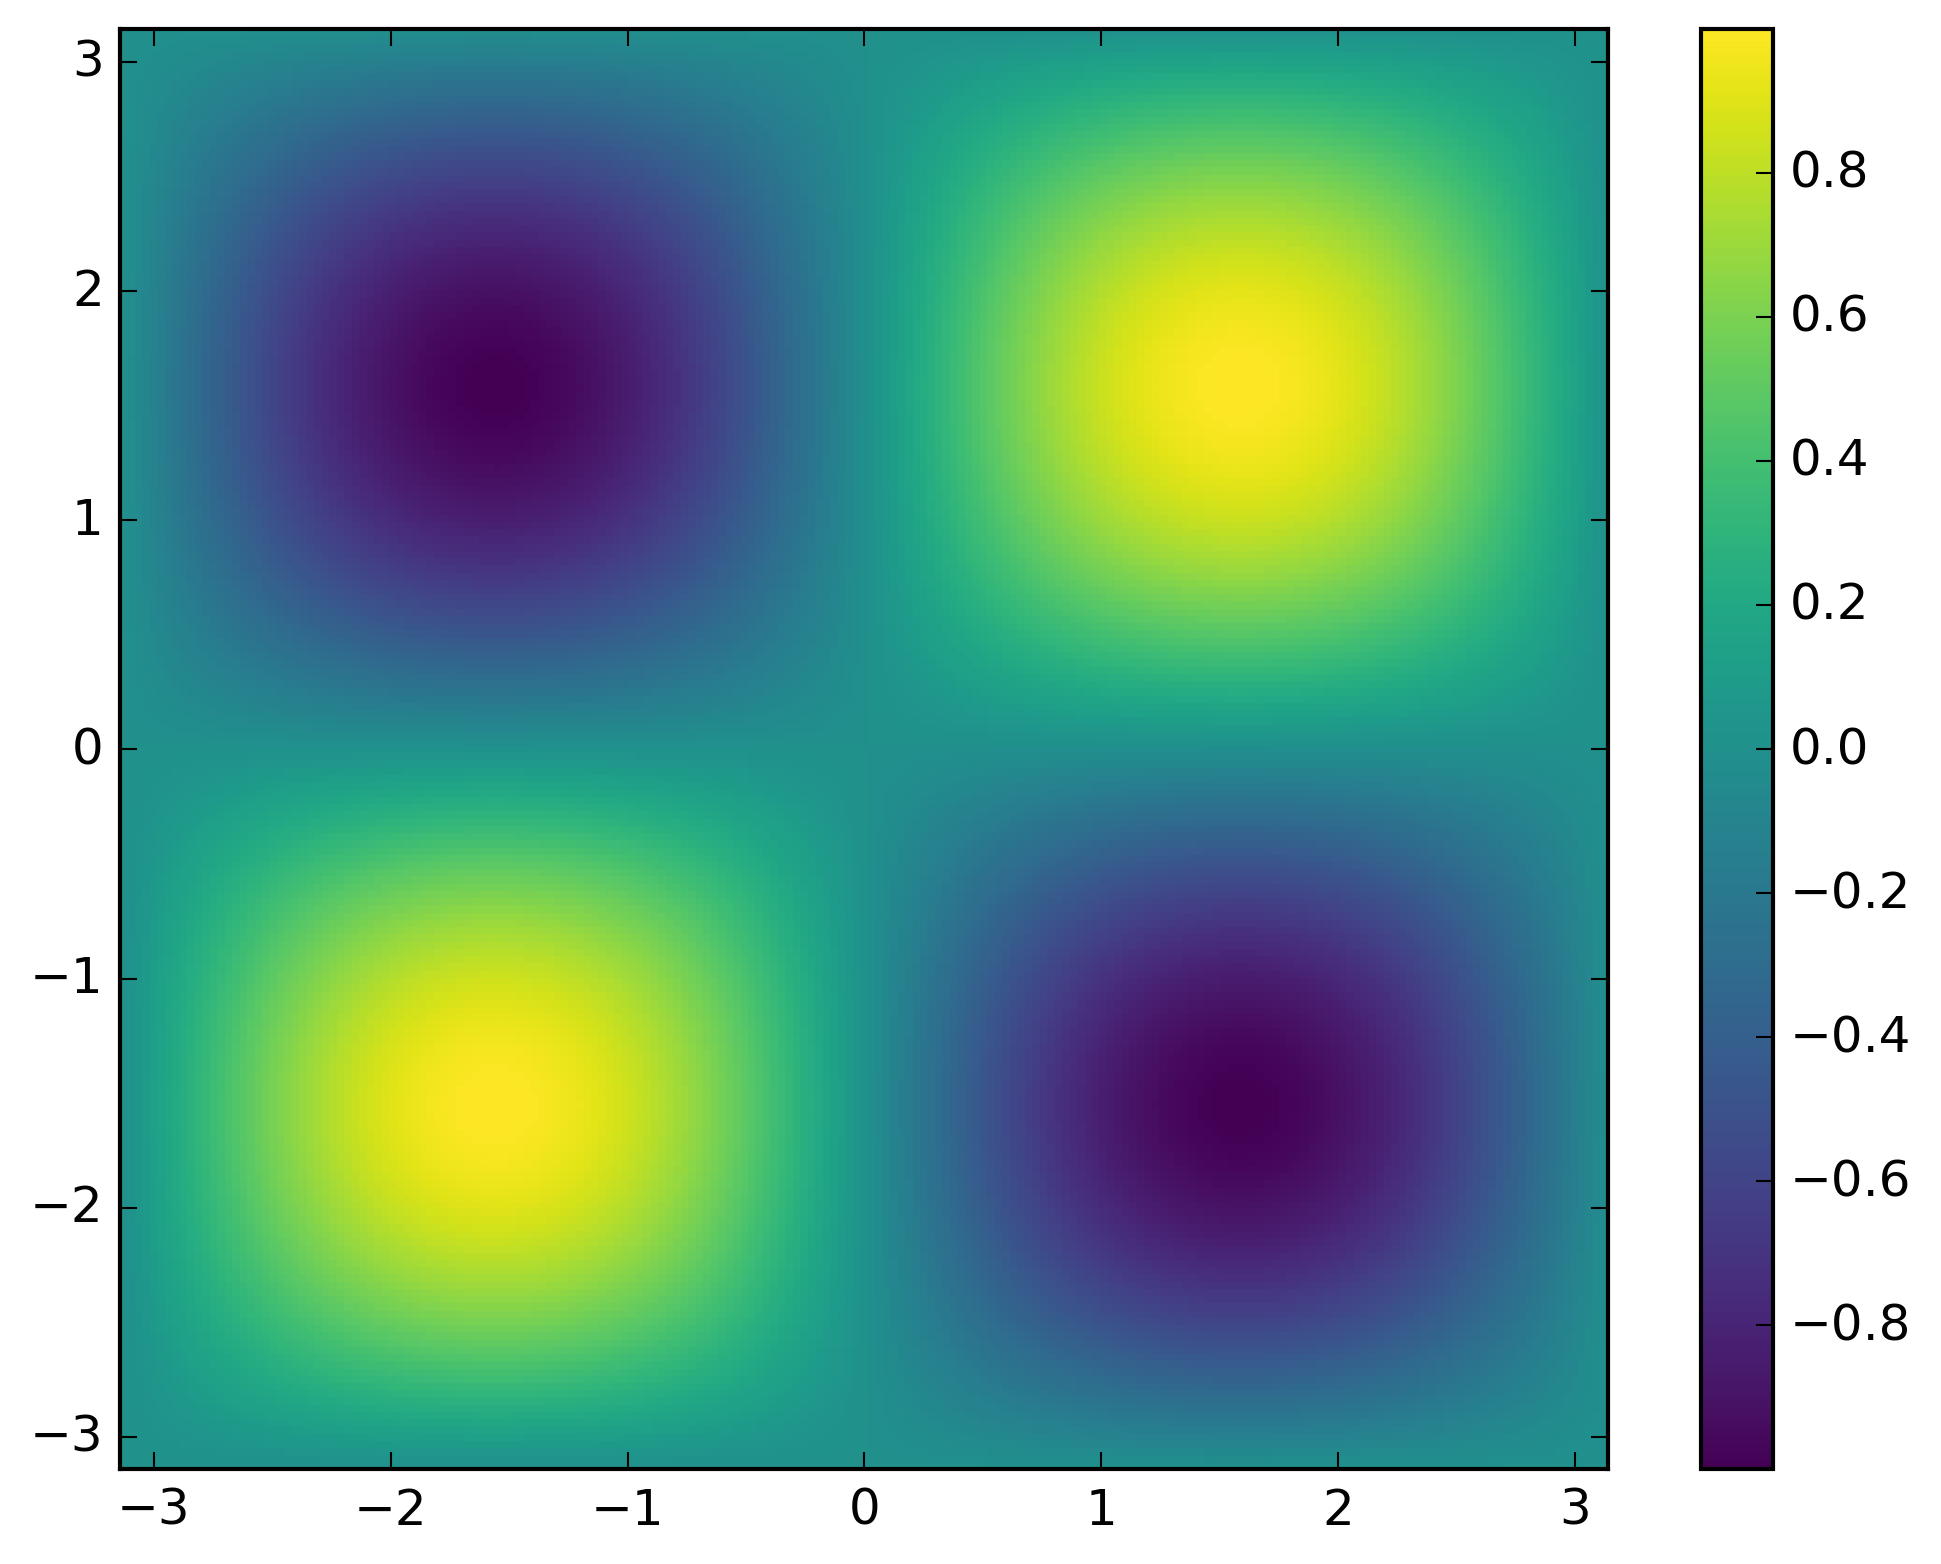
\includegraphics[width=\linewidth]{figures/heatmap.png}
\end{subfigure}%
\begin{subfigure}{.33\textwidth}
    \centering
    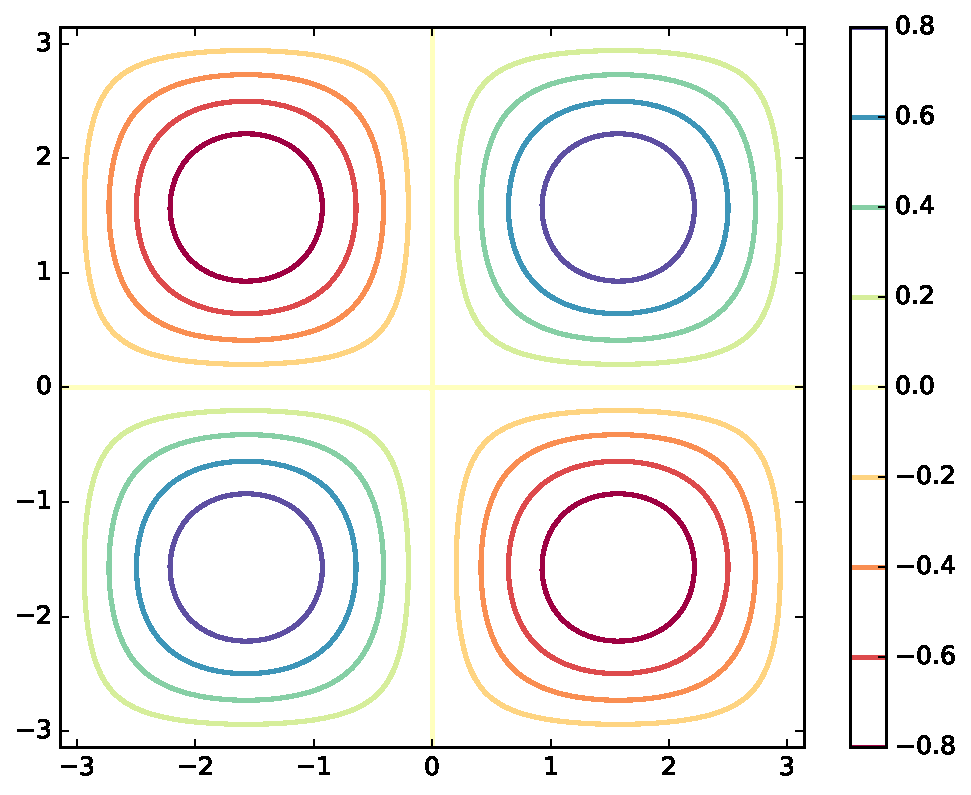
\includegraphics[width=\linewidth]{figures/contour.pdf}
\end{subfigure}%
\begin{subfigure}{.33\textwidth}
    \centering
    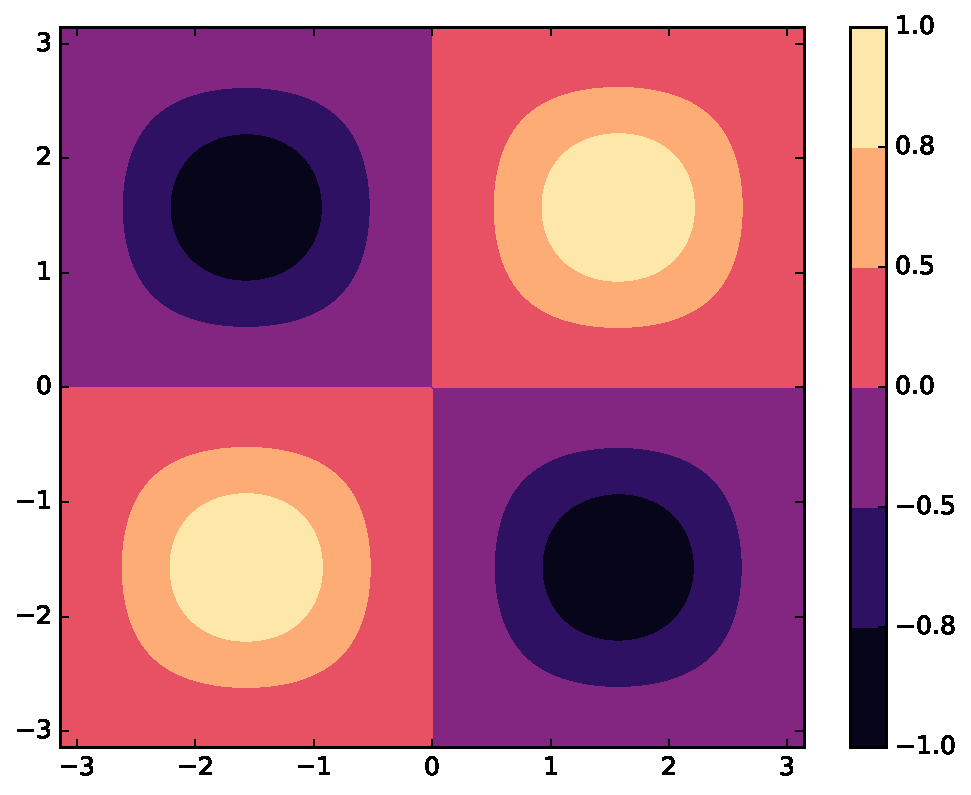
\includegraphics[width=\linewidth]{figures/contourf.pdf}
\end{subfigure}
\end{figure}

\begin{problem} % Heat map / contour plot of a function f:R2->R.
\label{prob:heatmap}
Write a function to plot $f(x,y) = \frac{\sin(x)\sin(y)}{xy}$ on the domain $[-2\pi,2\pi] \times [-2\pi,2\pi]$.

\begin{enumerate}
\item Create 2 subplots: one with a heat map of $f$, and one with a contour map of $f$.
Choose an appropriate number of level curves, or specify the curves yourself.
\item Set the limits of each subplot to $[-2\pi,2\pi] \times [-2\pi,2\pi]$.
\item Choose a non-default color scheme.
\item Include the color scale bar for each subplot.
\end{enumerate}
\end{problem}

\begin{info} % Note about plt.imshow().
Images are usually stored as either a 2-dimensional array (for black-and-white pictures) or a 3-dimensional array (a stack of 2-dimensional arrays, one for each RGB value).
This kind of data does not require a domain, and is easily visualized with \li{plt.imshow()}.
\end{info}

\newpage

\section*{Additional Material} % ==============================================

\subsection*{3-D Plotting} % --------------------------------------------------

Matplotlib can also be used to plot 3-dimensional surfaces.
The following code produces the surface corresponding to $f(x,y) = \sin(x)\sin(y)$.

\begin{lstlisting}
# Create the domain and calculate the range like usual.
>>> x = np.linspace(-np.pi, np.pi, 200)
>>> y = np.copy(x)
>>> X, Y = np.meshgrid(x, y)
>>> Z = np.sin(X)*np.sin(Y)

# Draw the corresponding 3-D plot using some extra tools.
>>> from mpl_toolkits.mplot3d import Axes3D
>>> fig = plt.figure()
>>> ax = fig.gca(projection='3d')
>>> ax.plot_surface(X, Y, Z)
>>> plt.show()
\end{lstlisting}

\begin{figure}[H]
    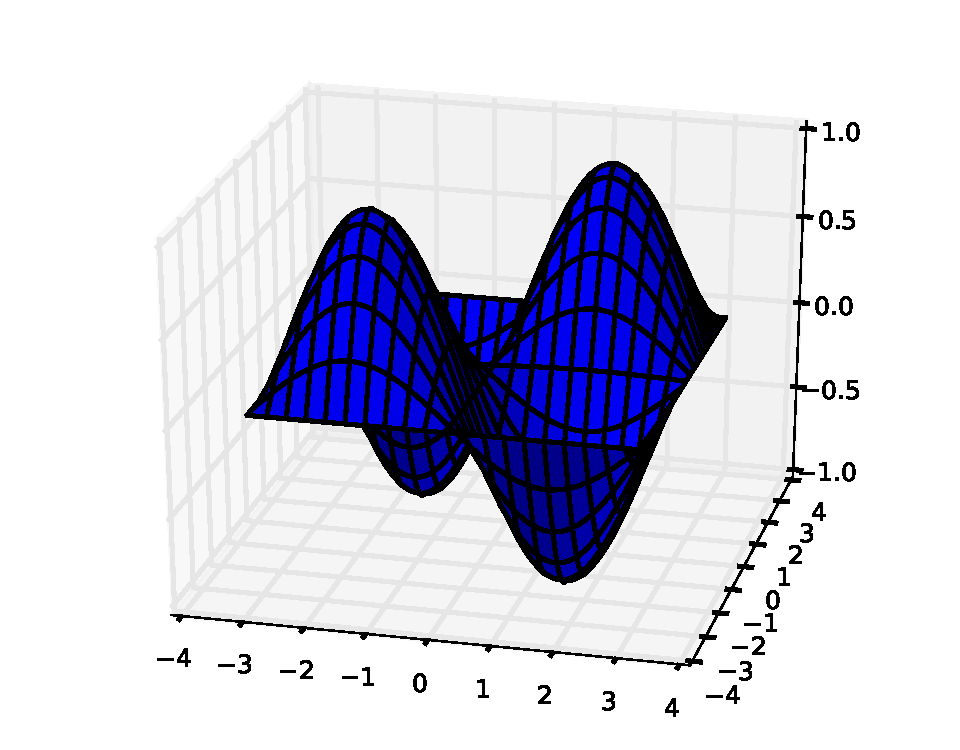
\includegraphics[width=.7\textwidth]{figures/surface_plot.pdf}
\end{figure}

\subsection*{Animations} % ----------------------------------------------------

Lines and other graphs can be altered dynamically to produce animations.
Follow these steps to create a Matplotlib animation:
%
\begin{enumerate}
    \item Calculate all data that is needed for the animation.
    \item Define a figure explicitly with \li{plt.figure()} and set its window boundaries.
    \item Draw empty objects that can be altered dynamically.
    \item Define a function to update the drawing objects.
    \item Use \li{matplotlib.animation.FuncAnimation()}.
\end{enumerate}

The submodule \li{matplotlib.animation} contains the tools putting together and managing animations.
The function \li{matplotlib.animation.FuncAnimation()} accepts the figure to animate, the function that updates the figure, the number of frames to show before repeating, and how fast to run the animation (lower numbers mean faster animations).

\begin{lstlisting}
from matplotlib.animation import FuncAnimation

def sine_animation():
    # Calculate the data to be animated.
    x = np.linspace(0, 2*np.pi, 200)[:-1]
    y = np.sin(x)

    # Create a figure and set its window boundaries.
    fig = plt.figure()
    plt.xlim(0, 2*np.pi)
    plt.ylim(-1.2, 1.2)

    # Draw an empty line. The comma after 'drawing' is crucial.
    drawing, = plt.plot([],[])

    # Define a function that updates the line data.
    def update(index):
        drawing.set_data(x[:index], y[:index])
        return drawing,                     # Note the comma!

    a = FuncAnimation(fig, update, frames=len(x), interval=10)
    plt.show()
\end{lstlisting}

Try using the following function in place of \li{update()}.
Can you explain why this animation is different from the original?

\begin{lstlisting}
def wave(index):
    drawing.set_data(x, np.roll(y, index))
    return drawing,
\end{lstlisting}

To animate multiple objects at once, define the objects separately and make sure the update function returns both objects.

\begin{lstlisting}
def sine_cosine_animation():
    x = np.linspace(0, 2*np.pi, 200)[:-1]
    y1, y2 = np.sin(x), np.cos(x)

    fig = plt.figure()
    plt.xlim(0, 2*np.pi)
    plt.ylim(-1.2, 1.2)

    sin_drawing, = plt.plot([],[])
    cos_drawing, = plt.plot([],[])

    def update(index):
        sin_drawing.set_data(x[:index], y1[:index])
        cos_drawing.set_data(x[:index], y2[:index])
        return sin_drawing, cos_drawing,

    a = FuncAnimation(fig, update, frames=len(x), interval=10)
    plt.show()
\end{lstlisting}

Animations are very useful for describing parametrized curves, as the ``speed'' of the curve is displayed.
The code below animates the rose curve, parametrized by the angle $\theta \in [0, 2\pi]$, given by the following equations:
%
\[\begin{array}{ccc}
x(\theta) = \cos(\theta)\cos(6\theta), && y(\theta) = \sin(\theta)\cos(6\theta)
\end{array}\]

\begin{lstlisting}
def rose_animation():
    # Calculate the parametrized data.
    theta = np.linspace(0, 2*np.pi, 200)
    x = np.cos(theta)*np.cos(6*theta)
    y = np.sin(theta)*np.cos(6*theta)

    fig = plt.figure()
    plt.xlim(-1.2, 1.2)
    plt.ylim(-1.2, 1.2)
    plt.gca().set_aspect("equal")           # Make the figure exactly square.

    drawing, = plt.plot([],[])

    # Define a function that updates the line data.
    def update(index):
        drawing.set_data(x[:index], y[:index])
        return drawing,

    a = FuncAnimation(fig, update, frames=len(x), interval=10, repeat=False)
    plt.show()              # repeat=False freezes the animation at the end.
\end{lstlisting}

Animations can also be 3-dimensional.
The only major difference is an extra operation to set the 3-dimensional component of the drawn object.
The code below animates the space curve parametrized by the following equations:
%
\[\begin{array}{ccccc}
x(\theta) = \cos(\theta)\cos(6\theta), &&
y(\theta) = \sin(\theta)\cos(6\theta), &&
z(\theta) = \frac{\theta}{10}
\end{array}\]

\begin{lstlisting}
def rose_animation_3D():
    theta = np.linspace(0, 2*np.pi, 200)
    x = np.cos(theta) * np.cos(6*theta)
    y = np.sin(theta) * np.cos(6*theta)
    z = theta / 10

    fig = plt.figure()
    ax = fig.gca(projection='3d')           # Make the figure 3-D.
    ax.set_xlim3d(-1.2, 1.2)                # Use ax instead of plt.
    ax.set_ylim3d(-1.2, 1.2)
    ax.set_aspect("equal")

    drawing, = ax.plot([],[],[])            # Provide 3 empty lists.

    # Update the first 2 dimensions like usual, then update the 3-D component.
    def update(index):
        drawing.set_data(x[:index], y[:index])
        drawing.set_3d_properties(z[:index])
        return drawing,

    a = FuncAnimation(fig, update, frames=len(x), interval=10, repeat=False)
    plt.show()
\end{lstlisting}

\begin{comment} % TODO: An ORIGINAL example of using widgets
\subsection*{Interactive Plots} % ---------------------------------------------

Matplotlib plots can be made interactive by adding \emph{widgets}.
Consider the following example, TAKEN FROM THE MATPLOTLIB DOCS BASICALLY AHHH

\begin{lstlisting}
>>> from matplotlib import widgets as wg

>>> ax = plt.subplot(111)
>>> plt.subplots_adjust(bottom=.25)         # Make some space for a slider bar.
>>> t = np.arange(0., 1., .001)
>>> a0 = 5.
>>> f0 = 3.
>>> s = a0 * np.sin(2 * np.pi * f0 * t)
>>> l = plt.plot(t, s)[0]
>>> plt.axis([0, 1, -10, 10])
>>> axfreq = plt.axes([.25, .05, .65, .03])
>>> axamp = plt.axes([.25, .1, .65, .03])

# Make some slider bars.
>>> sfreq = wg.Slider(axfreq, 'Freq', .1, 30., valinit=f0)
>>> samp = wg.Slider(axamp, 'Amp', .1, 10., valinit=a0)
>>> def update(val):                        # Function for updating the plot.
...     amp = samp.val                          # Read from one slider.
...     freq = sfreq.val                        # Read from the other slider.
...     l.set_ydata(amp * np.sin(2 * np.pi * freq * t))
...     plt.draw()                              # Refresh the plot.
>>> sfreq.on_changed(update)                # Connect the sliders to update().
>>> samp.on_changed(update)
>>> plt.show()
\end{lstlisting}

\begin{figure}[H]
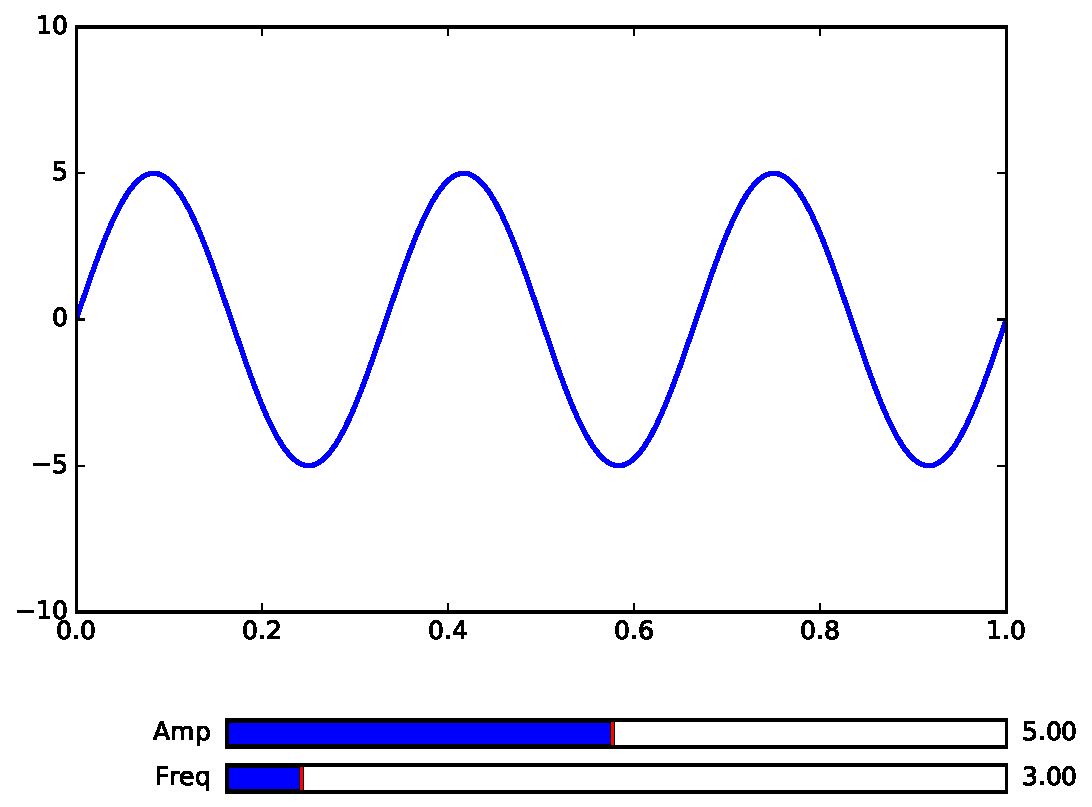
\includegraphics[width=.7\textwidth]{figures/interactive_plot.pdf}
\end{figure}
\end{comment}

% =============================================================================
% =============================================================================
% Stuff to move ===============================================================
% =============================================================================
% =============================================================================

\begin{comment}
\begin{info} % IPython Notebook inline plotting (move to notebook intro)
If you are executing these Matplotlib commands in an IPython shell, executing the \li{plt.show()} method will open a new window with the plot.
If you are using IPython Notebook, you have the option to display the plots within your notebook.
You may opt into this feature by running \li{\%matplotlib inline} or \li{\%matplotlib notebook} in your IPython Notebook.
The \li{inline} option shows the plot, whereas the \li{notebook} option shows the plot and provides controls to interact with the plot.
Additionally, when using this option, the plot is displayed after running the \li{plt.plot()} command; the \li{plt.show()} command is not necessary.
\end{info}
\end{comment}

